\chapter{Introduction}
 \section{Introduction}


DBMSs are widely used in many fields and find application in many companies as they provide relatively easy way of performing various operations on data, such as insertion, deletion, manipulation and update and at the same time they hide their internal complexity [2,3]. For this reason, applications can be implemented efficiently without worrying for handling low-level issues  such as concurrent access to data and efficient access which it is taken cared by DBMS. Hence, the main role of a DBMS is to store and manipulate data efficiently and consistently. Figure 1.1 shows in an abstract point of view the structure of modern DBMSs. Additionally, Structured Query language known as SQL is a standardised programming language for managing relational databases [1]. By having such standards, it can be provided an easily common interface for all DBMSs in order to manipulate and retrieve data from any given database without caring about the internal implementation. 


 \begin{figure} 
      \centering
      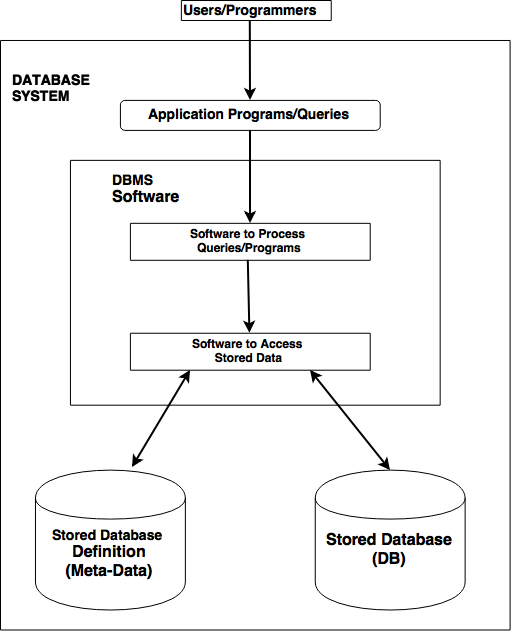
\includegraphics[width=\textwidth]{Images/Chapter1/db_arch}
      \caption{Abstract DBMS architecture}
      \label{fig:counting-methods}
    \end{figure}

  
As it was mentioned all current DBMSs currently support the SQL standards, meaning that there is a common language, namely SQL, that is used by all systems to manipulate data. Nevertheless some aspects of the standards are not well defined which make the process of interpret and implement it a difficult task and as a results, companies implement the SQL standards in a different manner. As a consequence programs that are written in SQL are partially portable among different DBMS.  

 \section{Motivation}
 SQL standards are set up for a long time, and they aim to provide a common use for modern DBMSs. As no specific DBMS predominates to each other, by studying in which extend various implementations differ in terms of their features that provide, is almost essential. These systems have been evolved rapidly, and new features are continuously added. As a result, many companies which use these systems, struggle to change their existing DBMS as their SQL code is not portable among other popular DBMSs. Hence, our initial goal is to have a tool to systematically discovers and highlight existing and new differences that may arise. Our tool will be used to evaluate five popular systems which are used by most companies, such as MySQL, IBM DB2, Microsoft SQL Server, PostgreSQL and Oracle Database. The results of this study will be significant for the vendors of the systems, users and companies that use these systems. Unfortunately, DBMSs do not always provide a meaningful message whenever an SQL code has a syntax error. As a consequence, it takes a time to detect and resolve the errors. By conducting this study, we intend to disclose all the incompatibilities that may exist.
 
 \section{Thesis Structure}
 The structure of the remainder of this thesis report is as follow: Chapter 2 provides an explanation about SQL language which is used with existing DBMSs and in addition it illustrates the main problem which should be investigated. Chapter 3 describes the main methodology that is used to investigate the problem. Chapter 4 gives a detailed explanation about the implementation. Chapter 5 presents our main findings and provide an explanation about the differences that exist between current DBMSs. Chapter 6 conclude this thesis project and provide ideas for future work.  

